% Options for packages loaded elsewhere
\PassOptionsToPackage{unicode}{hyperref}
\PassOptionsToPackage{hyphens}{url}
\PassOptionsToPackage{dvipsnames,svgnames*,x11names*}{xcolor}
%
\documentclass[
]{krantz}
\usepackage{lmodern}
\usepackage{amssymb,amsmath}
\usepackage{ifxetex,ifluatex}
\ifnum 0\ifxetex 1\fi\ifluatex 1\fi=0 % if pdftex
  \usepackage[T1]{fontenc}
  \usepackage[utf8]{inputenc}
  \usepackage{textcomp} % provide euro and other symbols
\else % if luatex or xetex
  \usepackage{unicode-math}
  \defaultfontfeatures{Scale=MatchLowercase}
  \defaultfontfeatures[\rmfamily]{Ligatures=TeX,Scale=1}
\fi
% Use upquote if available, for straight quotes in verbatim environments
\IfFileExists{upquote.sty}{\usepackage{upquote}}{}
\IfFileExists{microtype.sty}{% use microtype if available
  \usepackage[]{microtype}
  \UseMicrotypeSet[protrusion]{basicmath} % disable protrusion for tt fonts
}{}
\makeatletter
\@ifundefined{KOMAClassName}{% if non-KOMA class
  \IfFileExists{parskip.sty}{%
    \usepackage{parskip}
  }{% else
    \setlength{\parindent}{0pt}
    \setlength{\parskip}{6pt plus 2pt minus 1pt}}
}{% if KOMA class
  \KOMAoptions{parskip=half}}
\makeatother
\usepackage{xcolor}
\IfFileExists{xurl.sty}{\usepackage{xurl}}{} % add URL line breaks if available
\IfFileExists{bookmark.sty}{\usepackage{bookmark}}{\usepackage{hyperref}}
\hypersetup{
  pdftitle={Multimodal Deep Learning},
  colorlinks=true,
  linkcolor=Maroon,
  filecolor=Maroon,
  citecolor=Blue,
  urlcolor=Blue,
  pdfcreator={LaTeX via pandoc}}
\urlstyle{same} % disable monospaced font for URLs
\usepackage{longtable,booktabs}
% Correct order of tables after \paragraph or \subparagraph
\usepackage{etoolbox}
\makeatletter
\patchcmd\longtable{\par}{\if@noskipsec\mbox{}\fi\par}{}{}
\makeatother
% Allow footnotes in longtable head/foot
\IfFileExists{footnotehyper.sty}{\usepackage{footnotehyper}}{\usepackage{footnote}}
\makesavenoteenv{longtable}
\usepackage{graphicx,grffile}
\makeatletter
\def\maxwidth{\ifdim\Gin@nat@width>\linewidth\linewidth\else\Gin@nat@width\fi}
\def\maxheight{\ifdim\Gin@nat@height>\textheight\textheight\else\Gin@nat@height\fi}
\makeatother
% Scale images if necessary, so that they will not overflow the page
% margins by default, and it is still possible to overwrite the defaults
% using explicit options in \includegraphics[width, height, ...]{}
\setkeys{Gin}{width=\maxwidth,height=\maxheight,keepaspectratio}
% Set default figure placement to htbp
\makeatletter
\def\fps@figure{htbp}
\makeatother
\setlength{\emergencystretch}{3em} % prevent overfull lines
\providecommand{\tightlist}{%
  \setlength{\itemsep}{0pt}\setlength{\parskip}{0pt}}
\setcounter{secnumdepth}{5}
\usepackage{booktabs}
\usepackage{longtable}
\usepackage[bf,singlelinecheck=off]{caption}

\usepackage{framed,color}
\definecolor{shadecolor}{RGB}{248,248,248}

\renewcommand{\textfraction}{0.05}
\renewcommand{\topfraction}{0.8}
\renewcommand{\bottomfraction}{0.8}
\renewcommand{\floatpagefraction}{0.75}

\renewenvironment{quote}{\begin{VF}}{\end{VF}}
\let\oldhref\href
\renewcommand{\href}[2]{#2\footnote{\url{#1}}}

\makeatletter
\newenvironment{kframe}{%
\medskip{}
\setlength{\fboxsep}{.8em}
 \def\at@end@of@kframe{}%
 \ifinner\ifhmode%
  \def\at@end@of@kframe{\end{minipage}}%
  \begin{minipage}{\columnwidth}%
 \fi\fi%
 \def\FrameCommand##1{\hskip\@totalleftmargin \hskip-\fboxsep
 \colorbox{shadecolor}{##1}\hskip-\fboxsep
     % There is no \\@totalrightmargin, so:
     \hskip-\linewidth \hskip-\@totalleftmargin \hskip\columnwidth}%
 \MakeFramed {\advance\hsize-\width
   \@totalleftmargin\z@ \linewidth\hsize
   \@setminipage}}%
 {\par\unskip\endMakeFramed%
 \at@end@of@kframe}
\makeatother

\usepackage{makeidx}
\makeindex

\urlstyle{tt}

\usepackage{amsthm}
\makeatletter
\def\thm@space@setup{%
  \thm@preskip=8pt plus 2pt minus 4pt
  \thm@postskip=\thm@preskip
}
\makeatother

\frontmatter
\usepackage[]{natbib}
\bibliographystyle{apalike}

\title{Multimodal Deep Learning}
\author{}
\date{\vspace{-2.5em}2022-06-07}

\begin{document}
\maketitle

% you may need to leave a few empty pages before the dedication page

%\cleardoublepage\newpage\thispagestyle{empty}\null
%\cleardoublepage\newpage\thispagestyle{empty}\null
%\cleardoublepage\newpage
\thispagestyle{empty}

\begin{center}
\end{center}

\setlength{\abovedisplayskip}{-5pt}
\setlength{\abovedisplayshortskip}{-5pt}

{
\hypersetup{linkcolor=}
\setcounter{tocdepth}{0}
\tableofcontents
}
\hypertarget{preface}{%
\chapter*{Preface}\label{preface}}


\begin{figure}
\centering

\includegraphics{figures/by-nc-sa.png}
\caption{Creative Commons License}
\end{figure}

This book is licensed under the \href{http://creativecommons.org/licenses/by-nc-sa/4.0/}{Creative Commons Attribution-NonCommercial-ShareAlike 4.0 International License}.

\mainmatter

\hypertarget{foreword}{%
\chapter*{Foreword}\label{foreword}}


\emph{Author: Christoph Molnar}

This book is the result of an experiment in university teaching.
Each semester, students of the Statistics Master can choose from a selection of seminar topics.
Usually, every student in the seminar chooses a scientific paper, gives a talk about the paper and summarizes it in the form of a seminar paper.
The supervisors help the students, they listen to the talks, read the seminar papers, grade the work and then \ldots{} hide the seminar papers away in (digital) drawers.
This seemed wasteful to us, given the huge amount of effort the students usually invest in seminars.
An idea was born:
Why not create a book with a website as the outcome of the seminar?
Something that will last at least a few years after the end of the semester.
In the summer term 2019, some Statistics Master students signed up for our seminar entitled ``Limitations of Interpretable Machine Learning''.
When they came to the kick-off meeting, they had no idea that they would write a book by the end of the semester.

We were bound by the examination rules for conducting the seminar, but otherwise we could deviate from the traditional format.
We deviated in several ways:

\begin{enumerate}
\def\labelenumi{\arabic{enumi}.}
\tightlist
\item
  Each student project is part of a book, and not an isolated seminar paper.
\item
  We gave challenges to the students, instead of papers. The challenge was to investigate a specific limitation of interpretable machine learning methods.
\item
  We designed the work to live beyond the seminar.
\item
  We emphasized collaboration. Students wrote some chapters in teams and reviewed each others texts.
\end{enumerate}

\hypertarget{technical-setup}{%
\section*{Technical Setup}\label{technical-setup}}


The book chapters are written in the Markdown language.
The simulations, data examples and visualizations were created with R \citep{rlang}.
To combine R-code and Markdown, we used rmarkdown.
The book was compiled with the bookdown package.
We collaborated using git and github.
For details, head over to the \href{https://github.com/slds-lmu/seminar_multimodal_dl}{book's repository}.

\hypertarget{introduction}{%
\chapter{Introduction}\label{introduction}}

\emph{Author: }

\emph{Supervisor: }

\hypertarget{intro-about-the-seminar-topic}{%
\section{Intro About the Seminar Topic}\label{intro-about-the-seminar-topic}}

\hypertarget{outline-of-the-booklet}{%
\section{Outline of the Booklet}\label{outline-of-the-booklet}}

\hypertarget{chapter-1}{%
\chapter{Chapter 1}\label{chapter-1}}

\emph{Authors: Cem Akkus, Vladana Djakovic, Christopher Benjamin Marquardt}

\emph{Supervisor: Dr.~Matthias Aßenmacher}

Natural Language Processing (NLP) has existed for about 50 years, but it is more relevant than ever. There have been several breakthroughs in this branch of machine learning that is concerned with spoken and written language. For example, learning internal representations of words was one of the greater advances of the last decade. Word embeddings (\citet{Mikolov2013}, \citet{Bojanowski2016}) made it possible and allowed developers to encode words as dense vectors that capture their underlying semantic content. In this way, similar words are embedded close to each other in a lower-dimensional feature space. Another important challenge was solved by Encoder-decoder (also called sequence-to-sequence) architectures \citet{Sutskever2014}, which made it possible to map input sequences to output sequences of different lengths. They are especially useful for complex tasks like machine translation, video captioning or question answering. This approach makes minimal assumptions on the sequence structure and can deal with different word orders and active, as well as passive voice.

A definitely significant state-of-the-art technique is Attention \citet{Bahdanau2014}, which enables models to actively shift their focus -- just like humans do. It allows following one thought at a time while suppressing information irrelevant to the task. As a consequence, it has been shown to significantly improve performance for tasks like machine translation. By giving the decoder access to directly look at the source, the bottleneck is avoided and at the same time, it provides a shortcut to faraway states and thus helps with the vanishing gradient problem. One of the most recent sequence data modeling techniques is Transformers (\citet{vaswani2017attention}), which are solely based on attention and do not have to process the input data sequentially (like RNNs). Therefore, the deep learning model is better in remembering context-induced earlier in long sequences. It is the dominant paradigm in NLP currently and even makes better use of GPUs, because it can perform parallel operations. Transformer architectures like BERT (\citet{Devlin2018}), T5 (\citet{Raffel2019}) or GPT-3 (\citet{brown2020language}) are pre-trained on a large corpus and can be fine-tuned for specific language tasks. They have the capability to generate stories, poems, code and much more. With the help of the aforementioned breakthroughs, deep networks have been successful in retrieving information and finding representations of semantics in the modality text. In the next paragraphs, developments for another modality image are going to be presented.

Computer vision (CV) focuses on replicating parts of the complexity of the human visual system and enabling computers to identify and process objects in images and videos in the same way that humans do. In recent years it has become one of the main and widely applied fields of computer science. However, there are still problems that are current research topics, whose solutions depend on the research's view on the topic. One of the problems is how to optimize deep convolutional neural networks for image classification. The accuracy of classification depends on width, depth and image resolution. One way to address the degradation of training accuracy is by introducing a deep residual learning framework \citep{ResNet}. On the other hand, another less common method is to scale up ConvNets, to achieve better accuracy is by scaling up image resolution. Based on this observation, there was proposed a simple yet effective compound scaling method, called EfficientNets \citep{EfficientNet}.

Another state-of-the-art trend in computer vision is learning effective visual representations without human supervision. Discriminative approaches based on contrastive learning in the latent space have recently shown great promise, achieving state-of-the-art results, but the simple framework for contrastive learning of visual representations, which is called SimCLR, outperforms previous work \citep{SimCLR}. However, another research proposes as an alternative a simple ``swapped'' prediction problem where we predict the code of a view from the representation of another view. Where features are learned by Swapping Assignments between multiple Views of the same image (SwAV) \citep{SwAV}.
Further recent contrastive methods are trained by reducing the distance between representations of different augmented views of the same image (`positive pairs') and increasing the distance between representations of augmented views from different images (`negative pairs'). Bootstrap Your Own Latent (BYOL) is a new algorithm for self-supervised learning of image representatios \citep{BYOL}.

Self-attention-based architectures, in particular, Transformers have become the model of choice in natural language processing (NLP). Inspired by NLP successes, multiple works try combining CNN-like architectures with self-attention, some replacing the convolutions entirely. The latter models, while theoretically efficient, have not yet been scaled effectively on modern hardware accelerators due to the use of specialized attention patterns. Inspired by the Transformer scaling successes in NLP, one of the experiments is applying a standard Transformer directly to the image \citep{ImageT}. Due to the widespread application of computer vision, these problems differ and are constantly being at the center of attention of more and more research.

With the rapid development in NLP and CV in recent years, it was just a question of time to merge both modalities to tackle multi-modal tasks. The release of DALL-E 2 just hints at what one can expect from this merge in the future. DALL-E 2 is able to create photorealistic images or even art from any given text input. So it takes the information of one modality and turns it into another modality. It needs multi-modal datasets to make this possible, which are still relatively rare. This shows the importance of available data and the ability to use it even more. Nevertheless, all modalities are in need of huge datasets to pre-train their models. It's common to pre-train a model and fine-tune it afterwards for a specific task on another dataset. For example, every state-of-the-art CV model uses a classifier pre-trained on an ImageNet based dataset. The cardinality of the datasets used for CV is immense, but the datasets used for NLP are of a completely different magnitude. BERT uses the English Wikipedia and the Bookscorpus to pre-train the model. The latter consists of almost 1 billion words and 74 million sentences. The pre-training of GPT-3 is composed of five huge corpora: CommonCrawl, Books1 and Books2, Wikipedia and WebText2. Unlike language model pre-training that can leverage tremendous natural language data, vision-language tasks require high-quality image descriptions that are hard to obtain for free. Widely used pre-training datasets for VL-PTM are Microsoft Common Objects in Context (COCO), Visual Genome (VG), Conceptual Captions (CC), Flickr30k, LAION-400M and LAION-5B, which is now the biggest openly accessible image-text dataset.

Besides the importance of pre-training data, there must also be a way to test or compare the different models. A reasonable approach is to compare the performance on specific tasks, which is called benchmarking. A nice feature of benchmarks is that they allow us to compare the models to a human baseline. Different metrics are used to compare the performance of the models. Accuracy is widely used, but there are also some others. For CV the most common benchmark datasets are ImageNet, ImageNetReaL, CIFAR-10(0), OXFORD-IIIT PET, OXFORD Flower 102, COCO and Visual Task Adaptation Benchmark (VTAB). The most common benchmarks for NLP are General Language Understanding Evaluation (GLUE), SuperGLUE, SQuAD 1.1, SQuAD 2.0, SWAG, RACE, ReCoRD, and CoNLL-2003. VTAB, GLUE and SuperGLUE also provide a public leader board. Cross-modal tasks such as Visual Question Answering (VQA), Visual Commonsense Reasoning (VCR), Natural Language Visual Reasoning (NLVR), Flickr30K, COCO and Visual Entailment are common benchmarks for VL-PTM.

\hypertarget{title}{%
\section{title}\label{title}}

\emph{Author: }

\emph{Supervisor: }

\hypertarget{title-1}{%
\section{title}\label{title-1}}

\emph{Author: }

\emph{Supervisor: }

\hypertarget{resources-and-benchmarks-for-nlp-cv-and-multimodal-tasks}{%
\chapter{Resources and Benchmarks for NLP, CV and multimodal tasks}\label{resources-and-benchmarks-for-nlp-cv-and-multimodal-tasks}}

\emph{Author: Christopher Marquardt}

\emph{Supervisor: Prof.~Dr.~Christian Heumann}

Small Intro of my chapter

\begin{itemize}
  \item Explain that pre-training is huge part why NLP and CV models perform good
  \item Hint also that combination of both will be rest of the book
\end{itemize}

Intro for pretraining Ideas:

\begin{itemize}
  \item like an athlete. 
  \item Need some base fitness (=pre-training)
  \item Same like in reality pre-training differs between models. 
\end{itemize}

\subsection{Pre-training}
  \subsubsection{Resources for pre-training}
    \begin{itemize}
      \item how does pre-training look for NLP, CV, MML
      \item State and explain 3-4 of the most used resources (maybe add more)
      \item (How much effort to clean pre-training data)
      \item provide resources to find more (papers with code, ...)
      \item availability and size of pre-training for different modalities
        \begin{itemize}
          \item NLP > CV > MML (MML pretty new compared to others)
          \item Most of them not public (not good; Example JFT-300M)
          \item What role does size play (logarithmic)
        \end{itemize}
      \item How has pre-training changed or has it even changed in modalities
        \begin{itemize}
            \item CV: still all train on ImageNet ("Are we done with ImageNet") and poor performance of ObjectNet
            \item use of noisy data; ?quantity > quality?
          \end{itemize}
    \end{itemize}

\subsubsection{Use of resources}
    \begin{itemize}
      \item How pre-training is used in different modalities
        \begin{itemize}
          \item supervised
          \item self-supervised 
        \end{itemize}
        \item State and explain 2 or 3 main used pre-training tasks
          \begin{itemize}
            \item masked approaches
            \item ...
          \end{itemize}
      \end{itemize}

\subsection{Fine-tuning}
  \begin{itemize}
    \item why fine-tuning is important
    \item where and how to fine-tune
    \item ... 
  \end{itemize}

\subsection{Benchmarks for modalities}
  \begin{itemize}
    \item Importance of benchmarks
      \begin{itemize}
        \item also need for new ones (like Psych: Flynn Effect)
          \begin{itemize}
            \item do models get better or is it possible that pre-training                         contains already benchmarks (too much crawl; NLP)
          \end{itemize}
        \item Hint that models pre-train on different resources but perform on same benchmarks (good or bad)
        \end{itemize}
      \item different tasks for benchmarks
        \begin{itemize}
          \item state most important ones also give infor to find ohters (example: papers with code)
          \item Hint that it's most of the time reduction to classification tasks (like is this next sentences)
          \item Semantic of produced sentences often not nice
        \end{itemize}
  \end{itemize}

Outro: Multimodal architectures Chapter

\hypertarget{chapter-1-1}{%
\chapter{Chapter 1}\label{chapter-1-1}}

\emph{Authors: Author 1, Author 2}

\emph{Supervisor: Supervisor}

\hypertarget{lorem-ipsum}{%
\section{Lorem Ipsum}\label{lorem-ipsum}}

Lorem ipsum dolor sit amet, consetetur sadipscing elitr, sed diam nonumy eirmod tempor invidunt ut labore et dolore magna aliquyam erat, sed diam voluptua. At vero eos et accusam et justo duo dolores et ea rebum. Stet clita kasd gubergren, no sea takimata sanctus est Lorem ipsum dolor sit amet. Lorem ipsum dolor sit amet, consetetur sadipscing elitr, sed diam nonumy eirmod tempor invidunt ut labore et dolore magna aliquyam erat, sed diam voluptua. At vero eos et accusam et justo duo dolores et ea rebum. Stet clita kasd gubergren, no sea takimata sanctus est Lorem ipsum dolor sit amet.

\citet{rlang}

\hypertarget{using-figures}{%
\section{Using Figures}\label{using-figures}}

\begin{figure}

{\centering 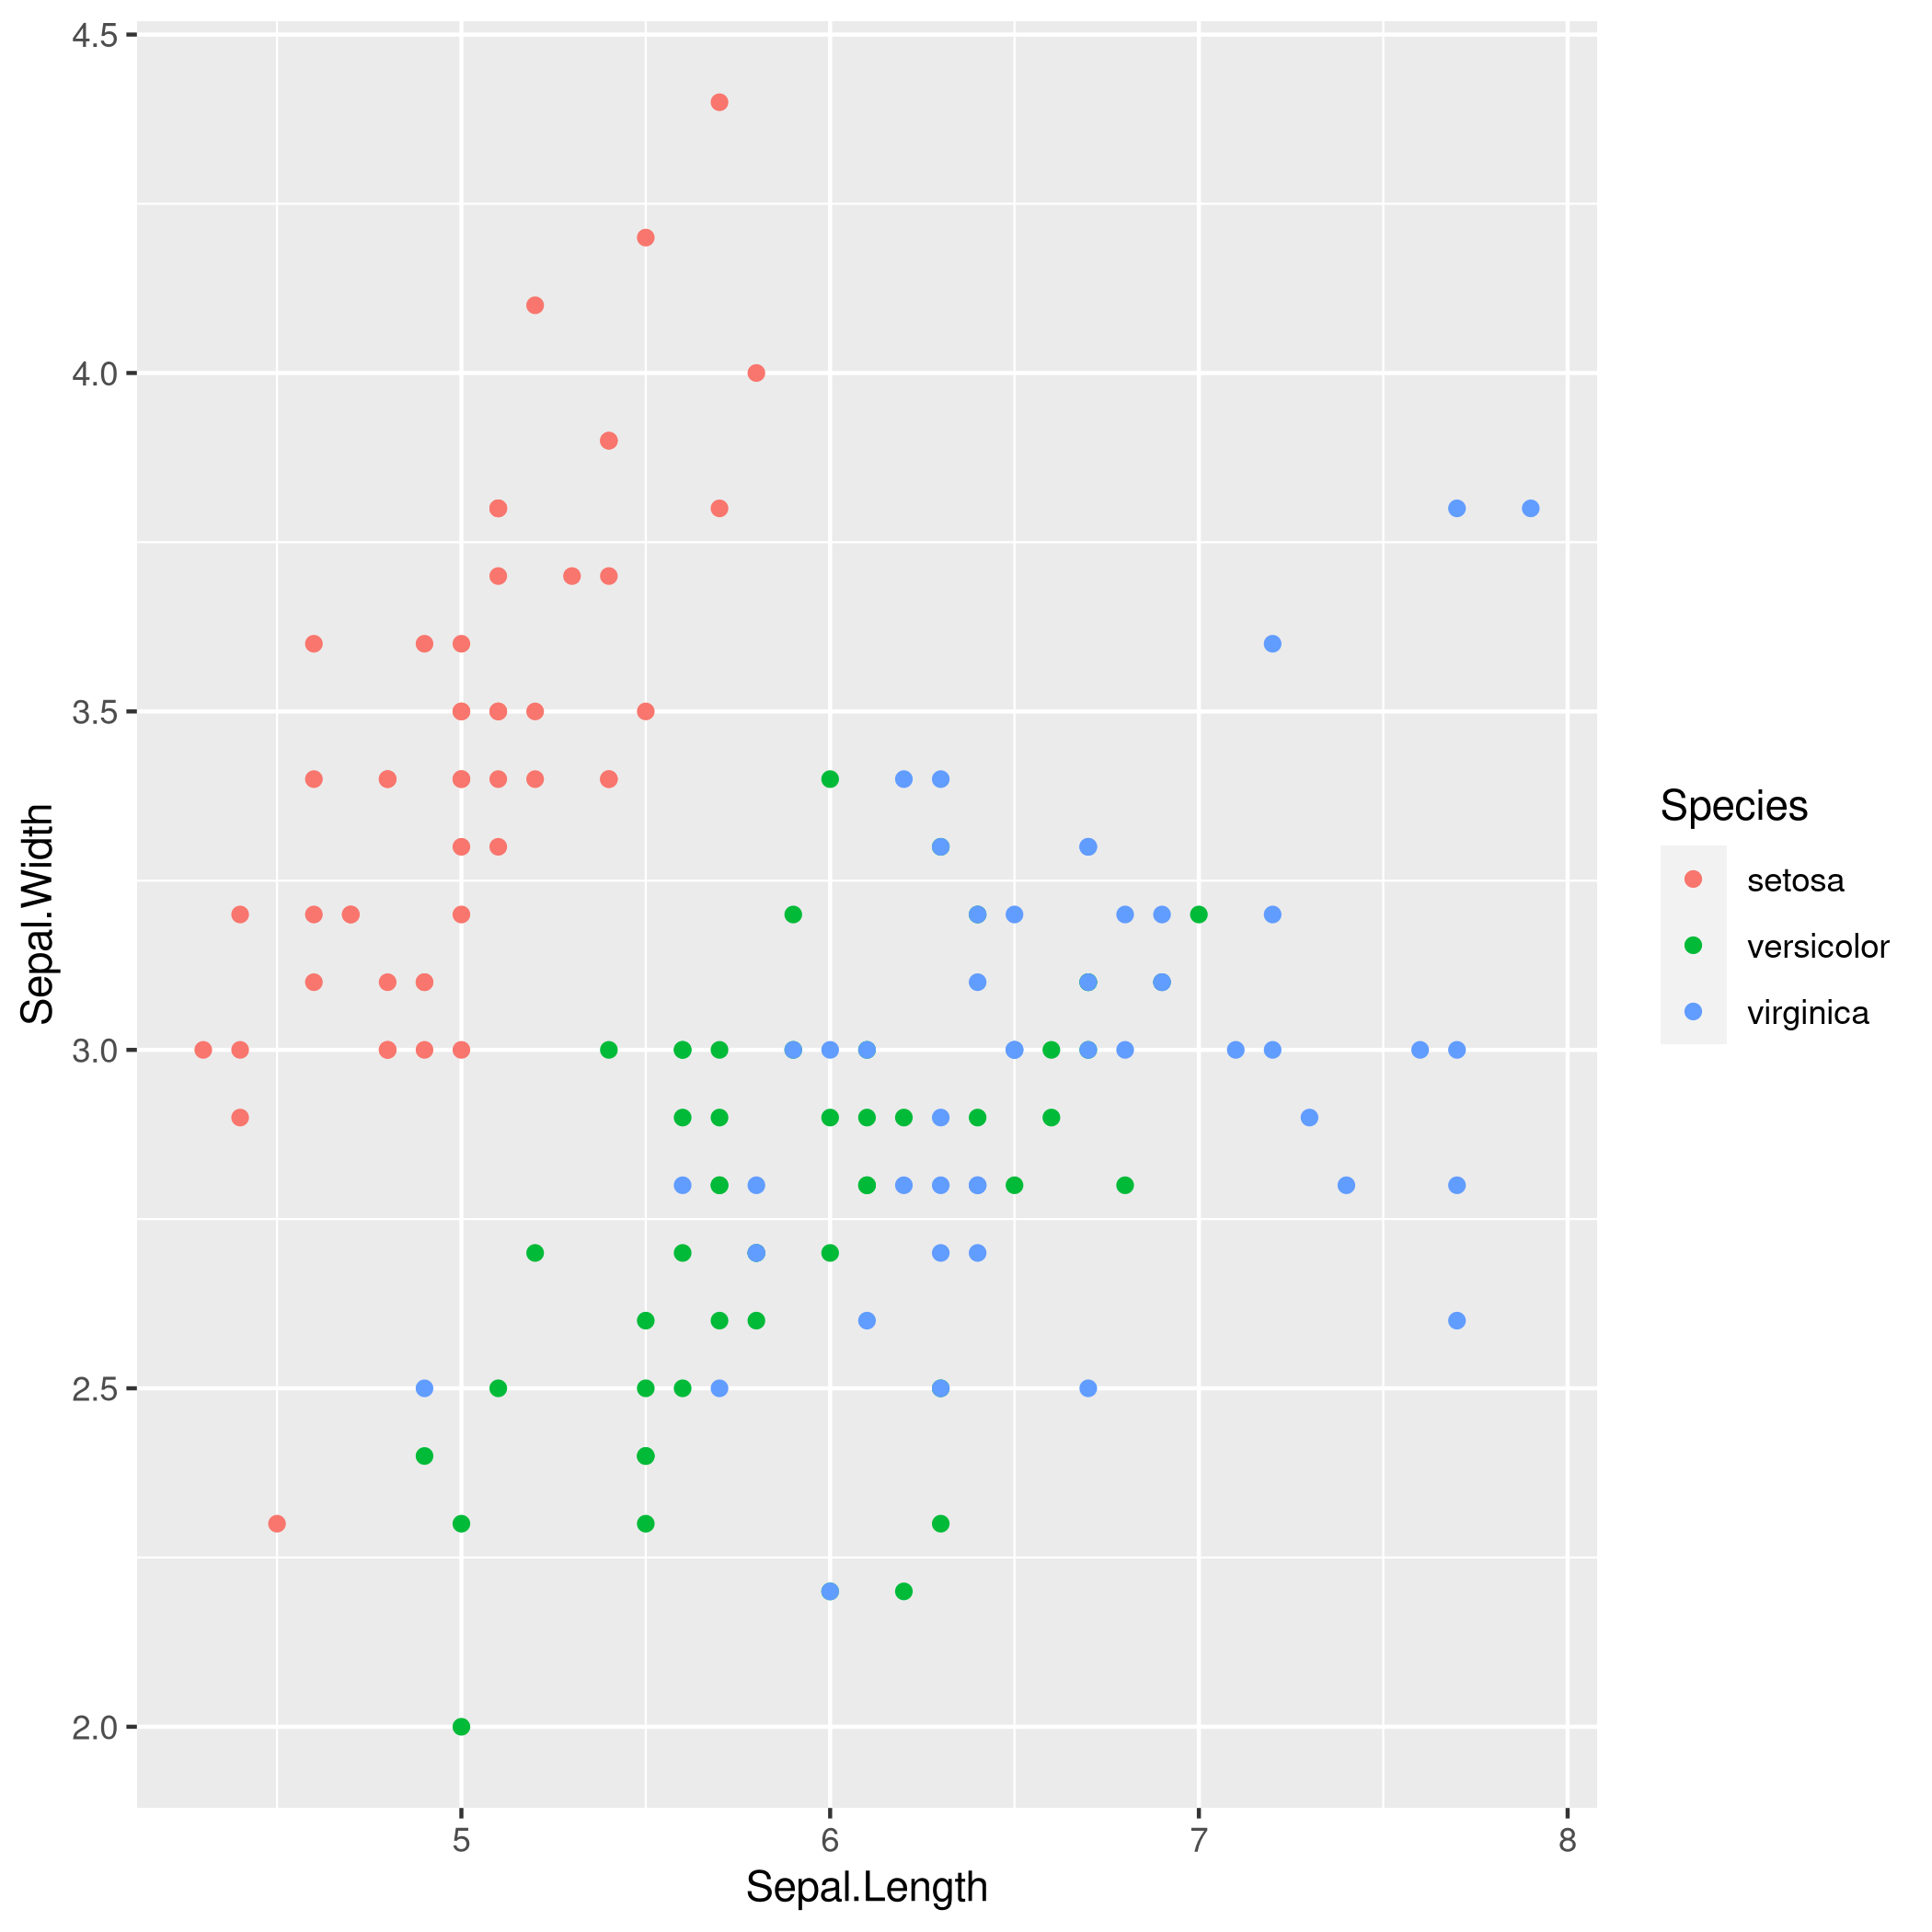
\includegraphics[width=0.8\linewidth]{figures/01-chapter1/ch01-figure01} 

}

\caption{This is the caption of the figure!}\label{fig:ch01-figure01-old}
\end{figure}



Referencing can be done by using the chunk label e.g.~\texttt{\textbackslash{}@ref(fig:ch01-figure01)} for \ref{fig:ch01-figure01}.

\textbf{NOTE!!!} Do not use underscores in chunk labels! This will crash the compilation \ldots{}

\hypertarget{using-tex}{%
\section{Using Tex}\label{using-tex}}

HTML rendering uses MathJax while pdf rendering uses LaTeX:

\[
f(x) = x^2
\]

\hypertarget{using-stored-results}{%
\section{Using Stored Results}\label{using-stored-results}}

\begin{tabular}{l|r|r|r|r}
\hline
  & Estimate & Std. Error & t value & Pr(>|t|)\\
\hline
(Intercept) & 2.1713 & 0.2798 & 7.760 & 0.0000\\
\hline
Sepal.Width & 0.4959 & 0.0861 & 5.761 & 0.0000\\
\hline
Petal.Length & 0.8292 & 0.0685 & 12.101 & 0.0000\\
\hline
Petal.Width & -0.3152 & 0.1512 & -2.084 & 0.0389\\
\hline
Speciesversicolor & -0.7236 & 0.2402 & -3.013 & 0.0031\\
\hline
Speciesvirginica & -1.0235 & 0.3337 & -3.067 & 0.0026\\
\hline
\end{tabular}

\hypertarget{title-2}{%
\chapter{title}\label{title-2}}

\emph{Author: }

\emph{Supervisor: }

\hypertarget{title-3}{%
\chapter{title}\label{title-3}}

\emph{Author: }

\emph{Supervisor: }

\hypertarget{title-4}{%
\chapter{title}\label{title-4}}

\emph{Author: }

\emph{Supervisor: }

\hypertarget{title-5}{%
\chapter{title}\label{title-5}}

\emph{Author: }

\emph{Supervisor: }

\hypertarget{title-6}{%
\chapter{title}\label{title-6}}

\emph{Author: }

\emph{Supervisor: }

\hypertarget{title-7}{%
\chapter{title}\label{title-7}}

\emph{Author: }

\emph{Supervisor: }

\hypertarget{chapter-2-multimodal-architectures}{%
\chapter{Chapter 2 Multimodal architectures}\label{chapter-2-multimodal-architectures}}

\emph{Authors: Luyang Chu, Karol Urbanczyk, Giacomo Loss, Max Schneider, Steffen Jauch-Walser}

\emph{Supervisor: Christian Heumann}

\hypertarget{introduction-1}{%
\section{Introduction}\label{introduction-1}}

Multimodal learning refers to the process of learning representations from different types of input modalities, such as image data, text or speech.
Due to methodological breakthroughs in the fields of Natural Language Processing (NLP) as well as Computer Vision (CV), in recent years multimodal models have gained increasing attention as they are able to strengthen predictions and better emulate the way humans learn.
This chapter focuses on discussing images and text as input data.
The remainder of the chapter is structured as follows:

The first part ``Image2Text'' discusses how transformer-based architectures improve meaningful captioning for complex images using a new large scale, richly annotated dataset COCO \citep{mccoco, cornia2020m2}.
Whether it is seeing a photograph and describing it or parsing a complex scene and describing its context, it is not a difficult task for humans.
But it is much more complex and challenging for computers.
We start with focusing on images as input modalities.
In 2014 Microsoft COCO was developed with a primary goal of advancing the state-of-the-art (SOTA) in object recognition by diving deeper into a broader question of scene understanding \citep{mccoco}.
COCO stands for Common Objects in Context.
It addresses three core problems in scene understanding: object detection (non-iconic views), segmentation, and captioning.
For tasks like machine translation and language understanding in NLP, transformer-based architecture is widely used.
However, the potential of these applications in the multi-modal context has not been fully covered.
With the help of the COCO dataset, a transformer-based architecture: Meshed-Memory Transformer for Image Captioning (\(M^2\)) will be introduced to improve both image encoding and the language generation steps \citep{cornia2020m2}.
The performance of the (\(M^2\)) Transformer and different fully-attentive models will be evaluated and compared on the COCO dataset.

Next, in ``Text2Image'', the idea of incorporating textual input in order to generate visual representations is described.
Current advancements in this field have been made possible largely due to recent breakthroughs in NLP, which first allowed for learning contextual representations of text.
Transformer-like architectures are being used to encode the input into embedding vectors, which are later helpful in guiding the process of image generation.
The chapter looks into details and discusses two SOTA model architectures by OpenAI, which both condition on text representations.
Surprisingly, none of them uses a GAN approach - a method which probably has been seen as the go-to idea for image generation over the last years.
The first model is DALL-E \citep{ramesh2021dalle}, which essentially combines Variational Encoder (VAE) with Autoregressive Transformer.
In the first step, VAE is being trained to learn downsized image representations.
Such embeddings are concatenated with text embeddings into one text-image pair input.
However, both of them use different dimensionality and vocabulary size.
In the second step, the transformer is trained on a next token prediction task given these data pairs.
Finally, at inference time, the model is able to generate images in the following way:

\begin{enumerate}
\def\labelenumi{\arabic{enumi}.}
\tightlist
\item
  Encode text input into text embedding
\item
  Use trained transformer from step 2 to generate image embedding
\item
  Use VAE from step 1 to generate image from image embedding
\end{enumerate}

The next approach to text-to-image generation is a GLIDE model \citep{nichol2021glide}.
GLIDE stands for Guided Language to Image Diffusion for Generation and Editing.
Its idea is to use Diffusion Models.
In its core, Diffusion Model is a simple idea -- random noise is being added to the image in an iterative fashion, and then model learns how to reconstruct this image.
In the case of GLIDE this learning process is conditioned on the text prompt, which is first passed through a transformer.
Both models differ in their results.
While DALL-E's resulting images might have been overwhelming back in the beginning of 2021, GLIDE is thought to significantly improve on photorealism and resolution the generated images.
Since the field has already seen further improvements following GLIDE, these new developments are also going to be mentioned in the chapter.

The third part, ``Images supporting Language Models'', deals with the integration of visual elements in pure textual language models.
Distributional semantic models such as Word2Vec and BERT assume that the meaning of a given word or sentence can be understood by looking at how (in which context) and when the word or the sentence appear in the text corpus, namely from its ``distribution'' within the text.
But this assumption has been historically questioned, because words and sentences must be grounded in other perceptual dimensions in order to understand their meaning \citep[see for example the ``symbol grounding problem'';][]{harnad1990symbol}.
For these reasons, a broad range of models has been developed with the aim to improve pure language models, leveraging on the addition of other perceptual information, such as visual ones.
This subchapter focuses in particular on the integration of visual elements (images) to support pure language models for various tasks at the word-level and sentence-level.
The starting point is always a language model, on which visual representations (extracted often with the help of large pools of images like MS COCO, see chapter ``Img2Text'' for further references) are to be ``integrated''.
But how?
There has been proposed a wide range of solutions:
On one side of the spectrum, textual elements and visual ones are learned separately and then ``combined'' together whereas on the other side, the learning of textual and visual features takes place simultaneously/jointly.

\begin{figure}

{\centering 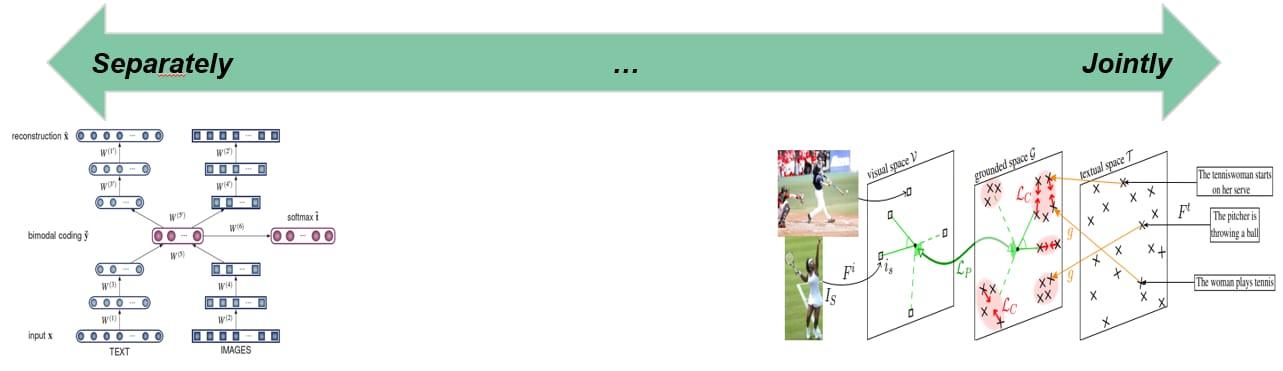
\includegraphics[width=1\linewidth]{figures/02-chapter2/Img_Ch_Intro} 

}

\caption{Left, Silberer et al., 2014: stacked autoencoders to learn higher-level embeddings from textual and visual modalities, encoded as vectors of attributes. Right, Bordes et al., 2020: textual and visual information fused in an Intermediate space denoted as “grounded space”; the “grounding objective function” is not applied directly on sentence embeddings but trained on this intermediate space, on which sentence embeddings are projected.}\label{fig:unnamed-chunk-1}
\end{figure}

For example, \citet{silberer2012grounded} implement a model where a one-to-one correspondence between textual and visual space is assumed.
Text and visual representations are passed to two separate unimodal encoders and both outputs are then fed to a bimodal autoencoder.
On the other side, \citet{bordes2020incorporating} propose a ``text objective function'' whose parameters are shared with an additional ``grounded objective function''.
The training of the latter takes place in what the authors called a ``grounded space'', which allows to avoid the one-to-one correspondence between textual and visual space.
These are just introductory examples and between these two approaches there are many shades of gray (maybe more than fifty\ldots).
These models exhibit in many instances better performance than pure language models, but they still struggle on some aspects, for example when they deal with abstract words and sentences.

Afterwards, in ``Text supporting Image Models'', approaches where natural language is used as supervision for CV models are described.
Intuitively these models should be more powerful compared to models supervised solely by manually labeled data, simply because there is much more training data available.
An important example for this is the CLIP model \citep{radford2021learning} with its new dataset WIT (WebImageText) comprising 400 million text-image pairs scraped from the internet.\\
Similar to ``Text2Image'' the recent successes in NLP have inspired new approaches in this field.
Most importantly pre-train methods, which directly learn from raw text \citep[e. g. GPT-n, Generative Pre-trained Transformer;][]{brown2020language}.
So, CLIP stands for Contrastive Language-Image Pre-training.
A transformer-like architecture is used for jointly pre-training a text encoder and an image encoder.
For this the contrastive goal to correctly predict which natural language text pertains to which image inside a certain batch, is employed.
Training this way turned out to be more efficient than to generate captions for images.\\
This leads to a flexible model, which at test time uses the learned text encoder as a ``zero-shot'' classifier on embeddings of the target dataset's classes.
The model, for example, can perform optical character recognition, geo-location and action-recognition.
Performance-wise CLIP can be competitive with task-specific supervised models, while never seeing an instance of the specific dataset before.
This suggests an important step towards closing the ``robustness gap'', where machine learning models fail to meet the expectations set by their previous performance -- especially on ImageNet test-sets -- on new datasets.

Finally, ``Text plus Images'' discusses how text and image inputs can be incorporated into a single unifying framework in order to get closer to a general self-supervised learning model.
There are two key advantages that make such a model particularly interesting.
Similar to models mentioned in previous parts, devoid of human labelling, self-supervised models don't suffer from the same capacity constraints as regular supervised learning models.
Nevertheless, while there have been notable advances in dealing with different modalities, it is often unclear to which extend a model structure generalizes across different modalities.
Rather than potentially learning modality-specific biases, a general multipurpose framework can help increase robustness while also simplifying the learner portfolio and thereby better emulating human learning processes.\\
Data2vec \citep{baevski2022data2vec} is a new multimodal self-supervised learning model which uses a single framework for either speech, NLP or computer vision.
This is in contrast to earlier models which used different algorithms for different modalities.
The core idea of data2vec, developed by MetaAI, is to predict latent representations of the full input data based on a masked view of the input in a self-distillation setup using a standard transformer architecture \citep{baevski2022data2vec}.
As a result, the main improvement is in the framework, not the underlying models themselves.
For example, the transformer architecture follows \citet{vaswani2017attention}.
Transformers have several advantages over CNNs, such as encoding the relative position of features (citation needed).
The central building block of the data2vec framework is a student-teacher structure that allows the learning process to occur without supervision.
To achieve this, inputs serve both as training data and as learning targets by being masked.
A key issue to be aware of is model collapse, i.e the model collapsing into a constant representation.
Normalization helps prevent that, as well as the domination of certain layers with high norm.
The encoding, normalization and masking strategies are modality-specific.
However, the learning objective remains the same across all modalities.
The model is trained to predict the model representation of the original unmasked training sample.
As a result of the use of self-attention in creating teacher representations, the data2vec model works with continuous and contextualized targets which are richer in information than a fixed set of targets based on local context as used in most prior work.
On top of that, working with latent representations of the network itself can be seen as a simplification of many prior modality-specific models \citep{baevski2022data2vec}.
As far as the results are concerned, data2vec is effective in all three modalities.
It sets new SOTA scores on computer vision, speech recognition as well as speech learning benchmarking sets.

\hypertarget{further-topics}{%
\chapter{Further Topics}\label{further-topics}}

\emph{Authors: Marco Moldovan, Rickmer Schulte, Philipp Koch}

\emph{Supervisor: Rasmus Hvingelby}

So far we have learned about multimodal models for text and 2D images. Text and images can be seen as merely snapshots of the sensory stimulus that we humans perceive constantly. If we view the research field of multimodal deep learning as a means to approach human-level capabilities of perceiving and processing real-world signals then we have to consider lots of other modalities in a trainable model other than textual representation of language or static images. Besides introducing further modalities that are frequently encountered in muli-modal deep learning, the following chapter will also aim to bridge the gap between the two fundamental sources of data, namely structured and unstructured data. Investigating modeling approaches from both classical statistics and more recent deep learning we will examine the strengths and weaknesses of those and will discover that a combination of both may be a promising path for future research. Going from multi modalities to multi task, the last section will then broaden our view of multi-modal deep learning by examining multi purpose modals. Discussing cutting-edge research topics such as the newly developed Pathways, we will discuss current achievements and limitations of the new modeling and hardware approaches that might lead our way towards the ultimate goal of AGI in multi-modal deep learning.

\hypertarget{further-modalities}{%
\chapter{Further Modalities}\label{further-modalities}}

\emph{Author: Marco Moldovan}

\emph{Supervisor: Rasmus Hvingelby}

\hypertarget{intro}{%
\section{Intro}\label{intro}}

In this chapter we will build up a taxonomy of different perceivable and interpretable types of signals that we as humans use to navigate the world and we will see how today's state-of-the-art multimodal models are built and trained in order to process more and more modalities simultaneously in order to build more and more complete representations of world through available data. We will build up our taxonomy starting from the two most well-understood modalities - namely text and 2D images - and introduce models that learn relationships between increasingly many modalities at the same time and to map them to a cross-modal representation space in which we can apply distance functions to points in order to represent semantic relatedness between datapoint from these different modalities.
Given such a learned cross-modal representation space we will look at some of the most important multimodal downstream tasks and applications.

Towards the end of the chapter we will take a closer look at the two main types of model architectures and training paradigms: bi-encoders and ``true'' multimodal cross-encoders. The first kind of model can be seen as an ensemble of unimodal expert models that map into the same representation space while using some form of metric learning to relate representations of different modalities to one another. True multimodal models are essentially agnostic to their input (as long as it is preprocessed and featurized appropriately). We currently see the second kind of architecture as the more promising one for the case of approximating human-level perception. An example of a modality agnostic multimodal model is the Perceiver of which we will introduce a newer, even more efficient variant.

Up until recently each modality required their own specific self-supervised training paradigm: for text a common approach would be MLM while the same training paradigm wasn't as effective for images or video. data2vec introduces a modality-agnostic SSL masked prediction setup which requires careful preprocessing but does not care about the source of the input. We see a model that marries a modality-agnostic model like Perceiver with a modality agnostic training paradigm like data2vec as a very promising path forward.
Topic 11 will build on this idea of modality-agnostic models by introducing Google's Pathways: a concept for multimodal, multi-task, sparse world models.

\hypertarget{strucutered-unstrucutered-data}{%
\chapter{Strucutered + Unstrucutered Data}\label{strucutered-unstrucutered-data}}

\emph{Author: Rickmer Schulte}

\emph{Supervisor: Daniel Schalk}

\hypertarget{intro-1}{%
\section{Intro}\label{intro-1}}

While the previous chapter has extended the range of modalities considered in multi-modal deep learning beyond image and text data, the focus remained on other sorts of unstructured data. This has neglected the broad class of structured data, which has been the basis for research in pre deep learning eras and which has given rise to many fundamental modeling approaches in statistics and classical machine learning. Hence, the following chapter will aim to give an overview of both data sources and outline the respective ways these have been used for modeling purposes as well as more recent attempts to model them jointly.

Generally, structured and unstructured data substantially differ in certain aspects such as dimensionality and interpretability which have led to various modeling approaches that are particularly designed for the special characteristics of the data types, respectively. As shown in previous chapters, deep learning models such as neural networks are known to work well on unstructured data due to their ability to extract latent representation and to learn complex dependencies from unstructured data sources to achieve state-of-the art performance on many classification and prediction tasks. By contrast, classical statistical models are mostly applied to tabular data due the advantage of interpretability inherent to these models, which is commonly of great interest in many research fields. However, as more and more data has become available to researchers today, they often do not only have one sort of data modality at hand but both structured and unstructured data at the same time. Discarding one or the other data modality makes it likely to miss out on valuable insights and potential performance improvements.

Therefore, the following chapter will mainly examine different concepts to model both data types jointly and discuss under which circumstances one or the other is better suited. Methods such as feature engineering to integrate unstructured data via expert knowledge into the classical model framework as well as different fusion strategies to integrate both types of modalities into common deep learning architectures are analyzed and evaluated. Especially the latter will be explored in detail by referring to numerous examples from health care, biology and finance. Finally, recently proposed methods will be discussed, which bring together classical statistical models for structured data and neural networks for unstructured data in order to yield interpretable deep learning models that combine the best of both worlds.

\hypertarget{multi-purpose-models}{%
\chapter{Multi-purpose Models}\label{multi-purpose-models}}

\emph{Author: Philipp Koch}

\emph{Supervisor: Rasmus Hvingelby}

\hypertarget{intro-2}{%
\section{Intro}\label{intro-2}}

After we describe further modalities in the previous sections, we will look at truly multipurpose models. Multitask multimodal models have already been proposed, like UniT, which extends the transformer architecture to deal with different modalities and tasks. However, previous multitask multimodal models remain limited in different aspects, which we will describe and discuss further. To become genuinely multipurpose, however, a model must be able to solve different tasks without fine-tuning and must be capable of dealing with different modalities. Thus, it must be able to transfer knowledge in-between tasks but must also be able to allocate capabilities for different modalities.

The recently introduced deep learning architecture Pathways is designed to be multipurpose. Pathways builds on newly designed hardware and software dedicated to addressing the challenges of contemporary deep learning models, which are ever-growing, where GPT-3 might be the most prominent example. We will discuss previous drawbacks and describe how Pathways aims to solve these issues. Besides the hardware aspect, Pathways provides a large neural network constructed as a directed acyclic graph (DAG). The input is passed through the network on different paths. Each node of the network is itself a neural network aimed at solving a specific aspect of a task. Using these different neural networks inside the model allows the model to be multitask and transfer knowledge in-between tasks. Another important aspect of this architecture is the obtained sparsity. When computed, just necessary nodes are computed, resulting in higher overall performance.

Furthermore, the model is intended to absorb different modalities as input, where no implementation has been found. Multimodality is further used hypothetically in the initial blog post. However, the similar model PathNet also achieves multimodality. The only model based on Pathways is the language model (PaLM), which is multilingual and capable of understanding code and solving mathematical tasks. However, the multimodality here remains questionable. Future Pathways-based models might provide more insight if the claim to step further toward artificial general intelligence (AGI) of the authors of Pathways and PathNet is true or not. Eventually, we will discuss the impact of the new Pathways multipurpose model since it might have a large impact on deep learning in the upcoming future. Broader applicable models will become feasible yet also centralize the usage, thus reducing accessibility and subsequently research on these models.

\hypertarget{title-8}{%
\chapter{title}\label{title-8}}

\emph{Author: }

\emph{Supervisor: }

\hypertarget{epilogue}{%
\chapter{Epilogue}\label{epilogue}}

\emph{Author: }

\hypertarget{test}{%
\section{test}\label{test}}

\hypertarget{acknowledgements}{%
\chapter{Acknowledgements}\label{acknowledgements}}

The most important contributions are from the students themselves.
The success of such projects highly depends on the students.
And this book is a success, so thanks a lot to all the authors!
The other important role is the supervisor.
Thanks to all the supervisors who participated!
Special thanks to \href{https://www.misoda.statistik.uni-muenchen.de/personen/professoren/heumann/index.html}{Christian Heumann} and \href{https://www.statistik.uni-muenchen.de/personen/professoren/bischl/index.html}{Bernd Bischl} who enabled us to conduct the seminar in such an experimental way, supported us and gave valuable feedback for the seminar structure.
Thanks a lot as well to the entire \href{https://www.statistik.uni-muenchen.de/}{Department of Statistics} and the \href{http://www.en.uni-muenchen.de/index.html}{LMU Munich} for the infrastructure.

The authors of this work take full responsibilities for its content.

  \bibliography{book.bib,packages.bib}

\backmatter
\printindex

\end{document}
